
\begin{figure}
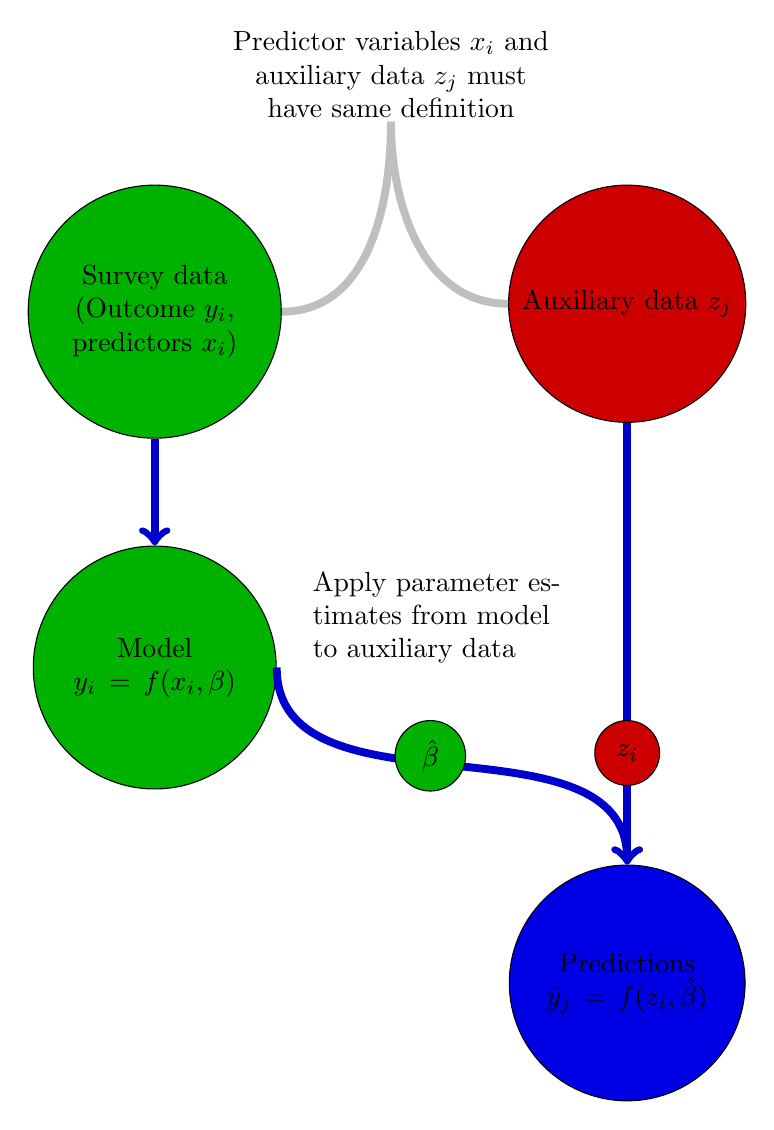
\begin{tikzpicture}[%
  % common options for blocks:
  block/.style = {draw, fill=blue!80!black, align=center, anchor=west,
              minimum height=0.65cm, inner sep=0},
  % common options for the circles:
  ball/.style = {circle, draw, align=center, anchor=north, inner sep=0}]
% Data sources
\node[ball,text width=3cm,fill=green!70!black] (survey) at (6,0) {Survey data (Outcome $y_i$, predictors $\boldsymbol{x}_i$)};
\node[ball,text width=3cm,fill=red!80!black] (aux) at (12,0) {Auxiliary data $\boldsymbol{z}_j$};

\node[anchor=north,text width=5cm,inner sep=.05cm,align=center,fill=white]
  (match) at (9,2) {Predictor variables $\boldsymbol{x}_i$ and auxiliary data $\boldsymbol{z}_j$ must have same definition};
\draw[-,line width=1mm,draw=gray!50] (survey.east) to [out=360,in=270] (match.south);
\draw[-,line width=1mm,draw=gray!50] (aux.west) to [out=180,in=270] (match.south);


\node[ball,fill=green!70!black,text width=3cm,anchor=base] (model) at (6,-6) {Model $y_i=f(\boldsymbol{x}_i, \boldsymbol{\beta})$};
\node[ball,fill=blue!90!black,text width=2.9cm,anchor=base] (preds) at (12,-10) {Predictions $\hat{y}_j = f(z_i, \hat{\boldsymbol{\beta}}$)};

% arrows showing split from all women to cancer and ~cancer
\draw[->,line width=1mm,draw=blue!80!black] (survey.south) to [out=270,in=90] (model.north);
\draw[->,line width=1mm,draw=blue!80!black] (model.east) to [out=270,in=90] (preds.north);
\draw[->,line width=1mm,draw=blue!80!black] (aux.south) to [out=270,in=90] (preds.north);


% transition from all women to actual cancer rates

% note illustration the p{cancer} circle (text won't fit inside)
\node[inner sep=0,anchor=west,text width=3.3cm] (note1) at (8,-5.5) {
   Apply parameter estimates from model to auxiliary data};
\node[ball,text width=.8cm,fill=green!70!black] (betahat) at (9.5,-6.8) {
   $\hat{\boldsymbol{\beta}}$};
\node[ball,text width=.8cm,fill=red!80!black] (z) at (12,-6.8) {
   $\boldsymbol{z}_i$};
\end{tikzpicture}
\label{sae_pic}
\caption{Basic outline of synthetic small area prediction}
\end{figure}

